\documentclass[12pt]{article}

\usepackage{orcidlink} % to insert a hyperlinked ORCiD logo
\usepackage{amssymb}
\usepackage{physics}
\usepackage{cite} % may be useful for different formats of numerical citation
\usepackage{hyperref} % for hyperlinks in references
\usepackage{caption} % for \caption*
\usepackage{amsmath}    % for "\eqref" macro
\usepackage{graphicx}











\textwidth 160mm
\textheight 230mm
\voffset = -20mm

\title{Thermodynamic response functions in a cell fluid model}

\author{O.A.Dobush, M.P.Kozlovskii, R.V.~Romanik
	\\ \small Institute for Condensed Matter Physics, NAS of Ukraine 
	\\ \small 1~Svientsitskii Street, 79011, Lviv, Ukraine 
	\\ \small romanik@icmp.lviv.ua}
%\author{R.V.~Romanik \\ Institute for Condensed Matter Physics, NAS of Ukraine}

\begin{document}
	
	\maketitle
	
	%\begin{multicols}{2}
	
	\abstract{Thermodynamic response functions, namely the isothermal compressibility, the thermal pressure coefficient, and the thermal expansion coefficient, are calculated for a many-particle system interacting through a modified Morse potential. These calculations are based on an equation of state previously derived for a cell fluid model in the grand canonical ensemble. The calculated quantities are presented graphically as functions of density and chemical potential.
	\\	
	\textbf{Keywords:} Simple fluids, Morse potential, Thermodynamic response functions.
	}
	\section{Introduction}
	
	In this work we continue our study of the thermodynamic behavior of a cell fluid model, which was defined in~\cite{KozitskyKozlovskiiDobush2018book,KozitskyKozlovskiiDobush2020}. In works~\cite{KozlovskiiDobush2020,PylyukDobush2020,PylyukEtAlJML2023,PylyukKozlovskiiDobushUJP2023b} this model was used with a modified Morse potential describing the particle interaction. In particular, the equation of state was obtained in~\cite{KozlovskiiDobush2020} in the zero-mode approximation. This equation of state is used in the current work to calculate thermodynamic response functions, namely the isothermal compressibility, the thermal pressure coefficient, and the thermal expansion coefficient.
	
	\section{The interaction potential}
	The potential of interaction between particles is taken in a form of a modified Morse potential
	\begin{equation}
		\label{def:mod_morse}
		U(r) = C_{H} \left[A {\rm e}^{-n_0(r-R_0)/\alpha} + {\rm e}^{-\gamma(r - R_0)/\alpha} -2{\rm e}^{-(r-R_0)/\alpha}\right],
	\end{equation}
	where $R_0$ is the coordinate of the potential minimum, $\alpha$ is an effective range of interaction, $\gamma$ and $n_0$ are parameters of the model. Other two constants $C_{H}$ and $A$ are expressed via $\gamma$ and $n_0$ as
	\begin{equation}
		C_{H} = \frac{\varepsilon n_0}{n_0 + \gamma - 2}, \quad A = \frac{2 - \gamma}{n_0},
	\end{equation}
	where $\varepsilon$ is the depth of the potential well at $r=R_0$. This potential is reduced to the ordinary Morse potential~\cite{Morse1929} at $\gamma=2$. For a more detailed discussion of such modified Morse potential, see Sections~1 and~2 in~\cite{KozlovskiiDobush2020}.
	
	Modifications of the Morse potential were used in other works as well. For example, in~\cite{MartinezValenciaEtAl2013} a repulsive term in a form of a power of $r^{-1}$ was added to the ordinary Morse potential, and the influence of the softness of such a term was investigated on the coordinates of the critical point. The generalized form of the Morse potential was suggested in~\cite{BiswasHamann1985}
	\begin{equation}
		U(r) = A_1 {\rm e}^{-\lambda_1 r} + A_2 {\rm e}^{-\lambda_2 r}
	\end{equation} 
	with application to silicon structural energies, and was also considered in~\cite{Lim2005} as the potential for Be-S and H-Na compounds.
	
	Our modification contains an additional repulsive term, similar to~\cite{MartinezValenciaEtAl2013}, as well as introduces parameter $\gamma$, which can vary as opposed to being strictly equal to 2 in the Morse potential. Including the repulsive term enables us to single out a reference system and apply the method of collective variables to calculating the grand partition function~[REFERENCE NEEDED].
	
	\section{The equation of state}
	The equation of state obtained in~\cite{KozlovskiiDobush2020} reads
	\begin{equation}
		\label{eq:eos}
		Pv\beta = E_\mu(M, T) + M \bar \rho_0 + \frac{1}{2} \tilde D(0) \bar \rho_0^2 - \frac{a_4}{24} \bar \rho_0^4.
	\end{equation}
	The quantities in the left-hand side of the equation are $P$, the pressure; $\beta$, the inverse temperature; $v$, cell volume. The quantities in the right-hand side are, in general, functions of the temperature $T$ and the chemical potential $\mu$. Let us present their expressions explicitly.
	
	First, the quantity $M$ depends linearly on the chemical potential
	\begin{align}\label{chem_pot}
		&	M = \frac{\tilde\mu}{W(0)} + g_1 + n_c \tilde D(0) - \frac{1}{6} \frac{g_3^3}{g_4^2}, \\
		&	\tilde\mu=\mu-\mu^*(1+\tau),
	\end{align}
	where $\mu^*$ is some positive constant, $\tau$ is the relative temperature $\tau = (T - T_c) / T_c$, $T_c$ is the critical temperature. We will call $M$ the effective chemical potential.
	
	The quantity $W(0)$ is expressed via parameters of the potential~(\ref{def:mod_morse}) as follows
	\begin{equation}
	W(0) = \Phi^{(r)}(0) \left[ B - 1 + \chi_0 + \tau (\chi_0 + A_\gamma) \right],
	\end{equation}
	where
	\begin{align} 
		& B = 2 \gamma^3 e^{(1-\gamma)/\alpha},\nonumber \\
		& A_\gamma = A e^{(n_0-\gamma)/\alpha} \left( \gamma / n_0\right)^3,
	\end{align}
	and $\Phi^{(r)}(0)$ is the Fourier transform of the repulsive part of the potential at $\abs{\vb k}=0$. The parameter $\chi_0$ is used in~\cite{KozlovskiiDobush2020} to single out a term in the Fourier transform of the potential that is treated as a reference system defined in the reciprocal space, and is selected as $\chi_0 = 0.07$.
	
	The coefficients $g_n$ are given by the formulas:
	\begin{align}
		& g_0 = \ln T_0, \qquad g_1 = T_1/T_0, \qquad g_2 = T_2/T_0 - g_1^2,  \nonumber \\
		& g_3 = T_3/T_0 - g_1^3 - 3g_1 g_2, \quad \qquad  g_4 = T_4/T_0 - g_1^4 - 6 g_1^2 g_2 - 4 g_1 g_3 - 3 g_2^2, \\
		& n_c = -g_3/g_4, \nonumber
	\end{align}
	where $T_n(p,\alpha^*)$ are the following special functions
	\begin{equation}
	T_n(p,\alpha^*) = \sum_{m=0}^{\infty} \frac{(\alpha^*)^m}{m!} m^n e^{pm^2}.
	\end{equation}
	Here $\alpha^*=v e^{\beta_c\mu^*}$, and the parameter $p$ has the form
	\begin{equation}
	p = \frac{\beta_c}{2} \Phi^{(r)}(0) [\chi_0 + A_\gamma].
	\end{equation} 
	The quantity $\beta_c$ denotes the critical value of the inverse temperature.
	Since $p$ is independent of temperature, the coefficients $g_n$ are also independent of temperature. The numerical values for other coefficients used in this paper are the same as those in~\cite{KozlovskiiDobush2020}:
	\begin{equation*}
		\alpha^* = 5.0, \quad \gamma = 1.65, \quad n_0 = 1.521.
	\end{equation*}
	
	The quantity $\tilde D(0)$ entering equations~\eqref{eq:eos} and~\eqref{chem_pot} is a function of temperature
	\begin{equation}
	\tilde D(0) = g_2 - \frac{1}{2} \frac{g_3^2}{g_4} - \frac{1}{\beta W(0)}.
	\end{equation}
	The condition $\tilde{D}(0) = 0$ defines the critical temperature~\cite{KozlovskiiDobush2020}
	\begin{equation}
		T_c = \left(g_2 - \frac{1}{2} \frac{g_3^2}{g_4} \right) (B - 1 + \chi_0) \Phi^{(r)}(0).
	\end{equation}    
	
	The function $E_\mu(M, T)$ from the equation \eqref{eq:eos} is provided by
	\begin{align}
		& E_\mu (M, T) = - \frac{1}{2 N_v} \ln (2\pi \beta W(0)) +  g_0 - \frac{\beta W(0)}{2} \!\! \left( \! \frac{\tilde\mu}{W(0)} \! \right)^{\! 2} \!\!\! - \frac{g_3}{g_4} {M} \! - \frac{g_3^2}{2 g_4^2}  \tilde D(0) - \frac{1}{24} \frac{g_3^4}{g_4^3}. 
	\end{align}
	Note that for all $ \tau> 0 $ there are no restrictions on the value of $ \bar \rho_0 $, which is a function of the temperature and the chemical potential
	\begin{equation}\label{2d18}
	\bar \rho_0 = \left(- \frac{3\bar{M}}{g_4} + \sqrt{Q_t}\right)^{1/3} - \left(  \frac{3\bar{M}}{g_4} + \sqrt{Q_t} \right)^{1/3} \!\!\!\! ,
	\end{equation}
	where
	\begin{equation}
	Q_t = \left(  \frac{2\tilde D(0)}{g_4}\right)^3 + \left( -\frac{3\bar{M}}{g_4}\right)^2, \qquad g_4<0.
	\end{equation}  
	...
	\begin{equation}\label{3d3}
	\bar n = n_g - \bar{M} + \tilde g_2 \gamma_\tau \bar \rho_0,
	\end{equation}
	where
	\begin{equation}\label{3d4}
	n_g = g_1 + n_c \tilde g_2 - \frac{1}{6} g_3^3 / g_4^2.
	\end{equation}
	...
	
	Figure~1 shows the isotherms for the pressure $P$ following from the equation of state~(\ref{eq:eos})
	\begin{figure}[h!]
		%\centering 
		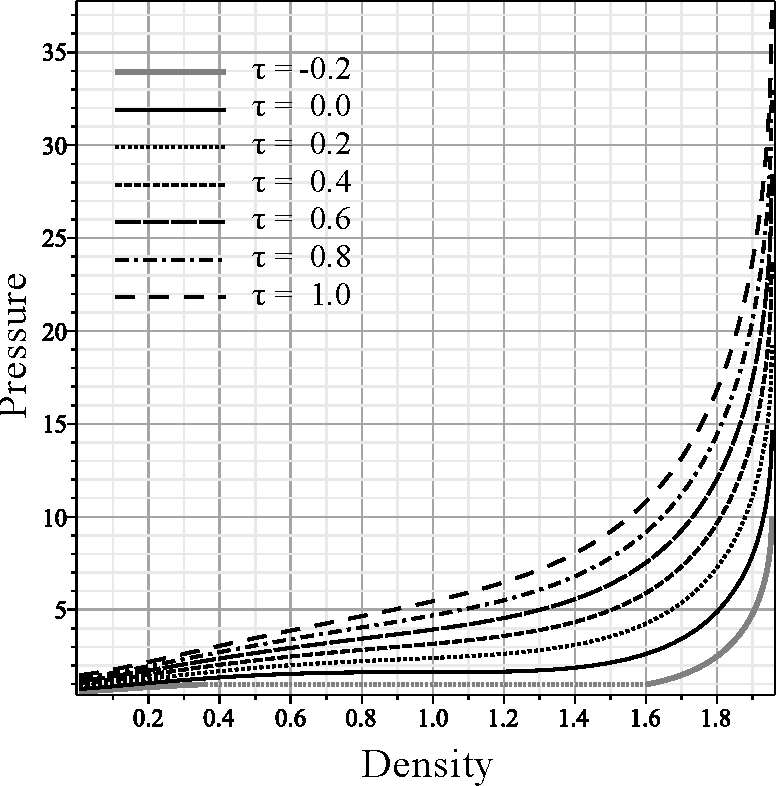
\includegraphics[width=0.446\textwidth]{f1a1.pdf} 
		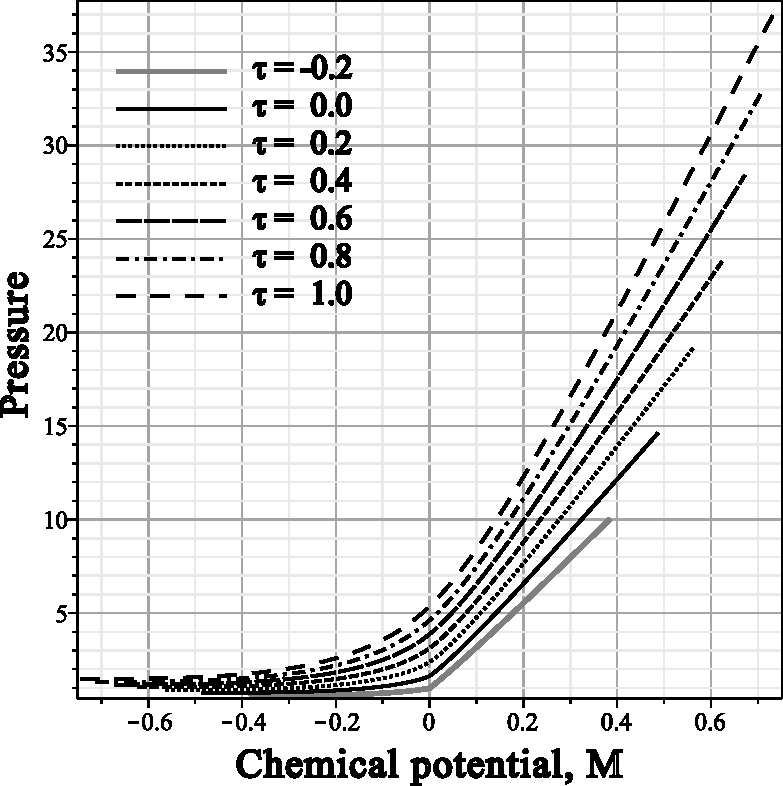
\includegraphics[width=0.45\textwidth]{f1b1.pdf} 
		\vskip-3mm\caption{Plots of isotherms of the pressure $P$ as a function of the density $\bar n$ (on the lefthand side) and a function of the effective chemical potential $M$ (on the righthand side) at $T \geq T_c$ represented by black lines. Thick grey lines on both figures correspond to isotherms of pressure at $T < T_c$ based on the results taken from~\cite{KozlovskiiDobush2020}. 
		}\label{fig1}
	\end{figure}
	
	\section{Thermodynamic response functions (coefficients)}
	
	\subsection{Isothermal compressibility}
	The isothermal compressibility is defined by
	\begin{equation}
		\label{def:isotherm_compres}
		K_T = -\frac{1}{V}\left(\frac{\partial V}{\partial P}\right)_{T,<N>}
	\end{equation}
	
	\begin{figure}[h!]
		\centering 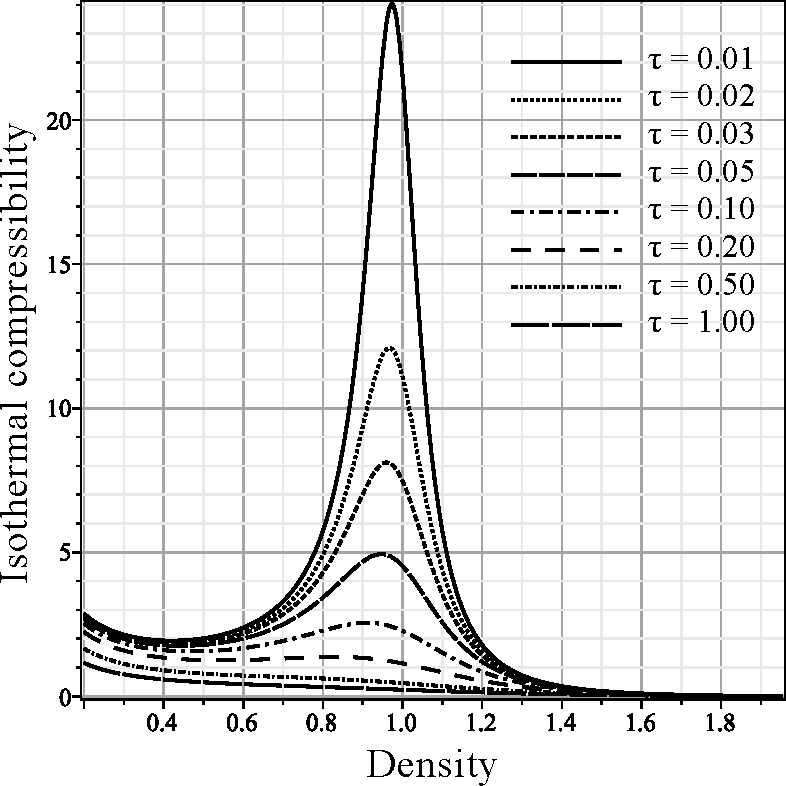
\includegraphics[width=0.5\textwidth]{f2a.pdf}
		\vskip-3mm\caption{The isothermal compressibility $K_T$ as a function of the density $\bar n$ at different values of reduced temperature $\tau > 0$ ($T > T_c$). 
		}\label{fig2a}
	\end{figure}
	
	\begin{figure}[h!]
		\centering 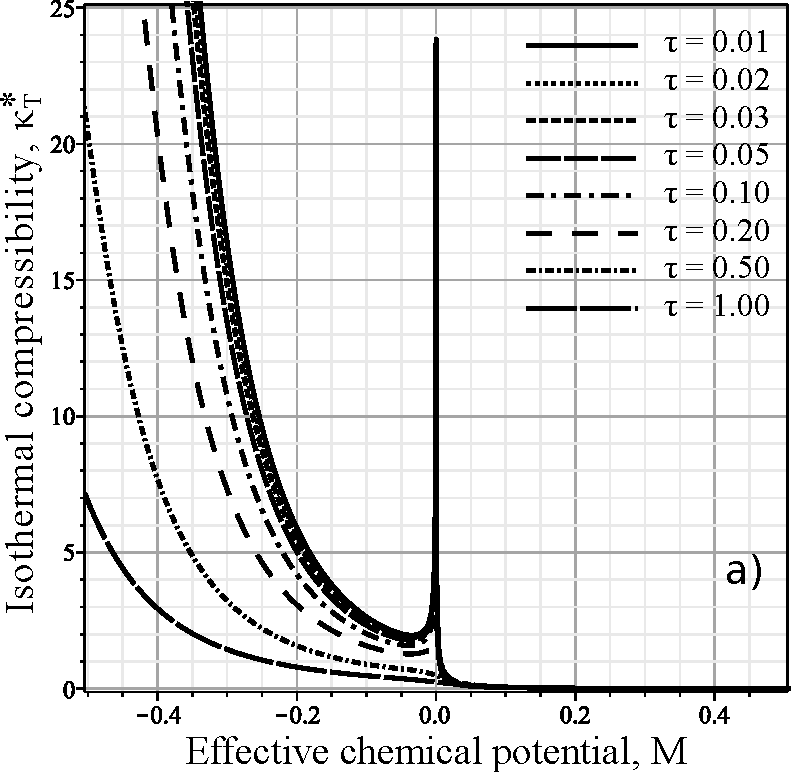
\includegraphics[width=0.45\textwidth]{f2b.pdf}
		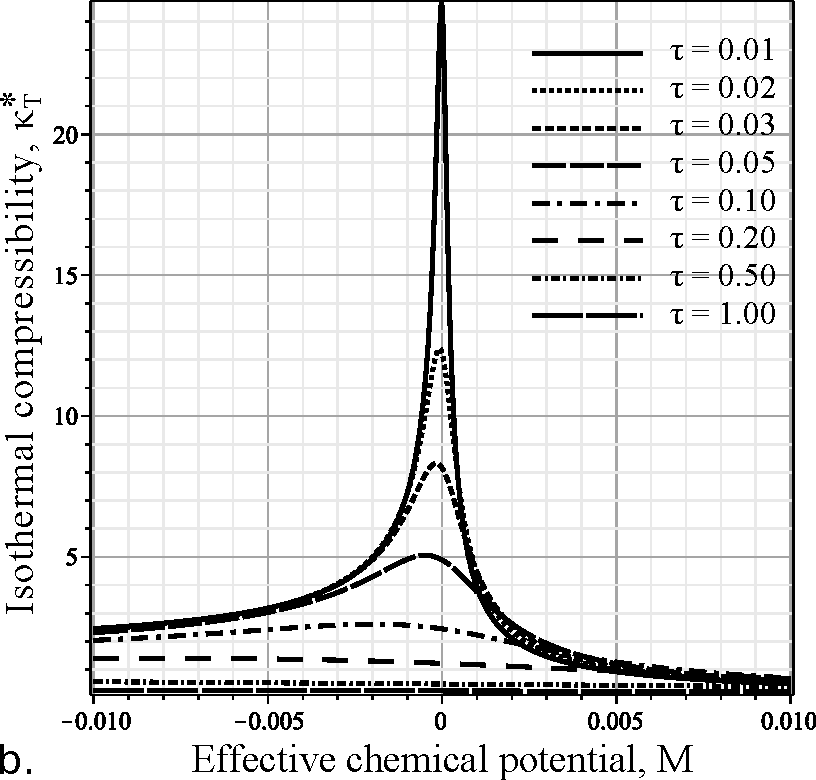
\includegraphics[width=0.475\textwidth]{f2c.pdf}
		\vskip-3mm\caption{The isothermal compressibility $K_T$ as a function of the effective chemical potential $M$ for different temperatures $\tau = (T - T_c)/T_c$ at $T > T_c$. The two figures differ in the scale of $M$. The left-hand-side figure covers a wider range of $M$, while the right-hand-side one focuses on a range of $M$ around its critical value $0$.
		}\label{fig2b}
	\end{figure}
	
	\subsection{Thermal pressure coefficient}
	The thermal pressure coefficient is defined by
	\begin{equation}
		\label{def:therm_pres_coef}
		\beta_V = \left( \frac{\partial P}{\partial T} \right)_{V,<N>}
	\end{equation}
	
	\begin{figure}[h!]
		\centering 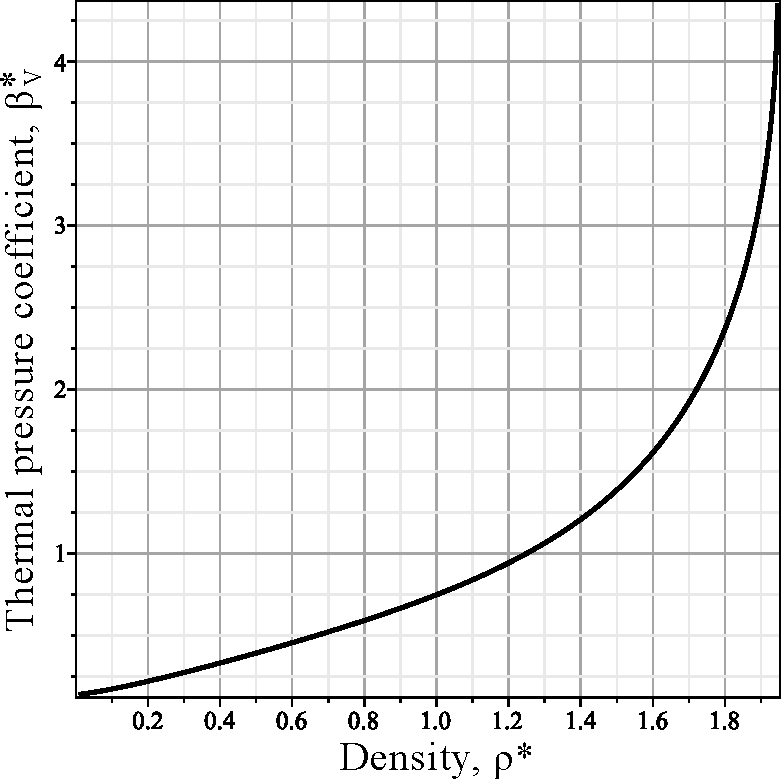
\includegraphics[width=0.5\textwidth]{f3a.pdf}
		\vskip-3mm\caption{The thermal pressure coefficient $\beta_V$ as a function of the density $\bar n$ at different values of relative temperature $\tau > 0$ ($T > T_c$). 
		}\label{fig3a}
	\end{figure}
	\begin{figure}[h!]
		\centering 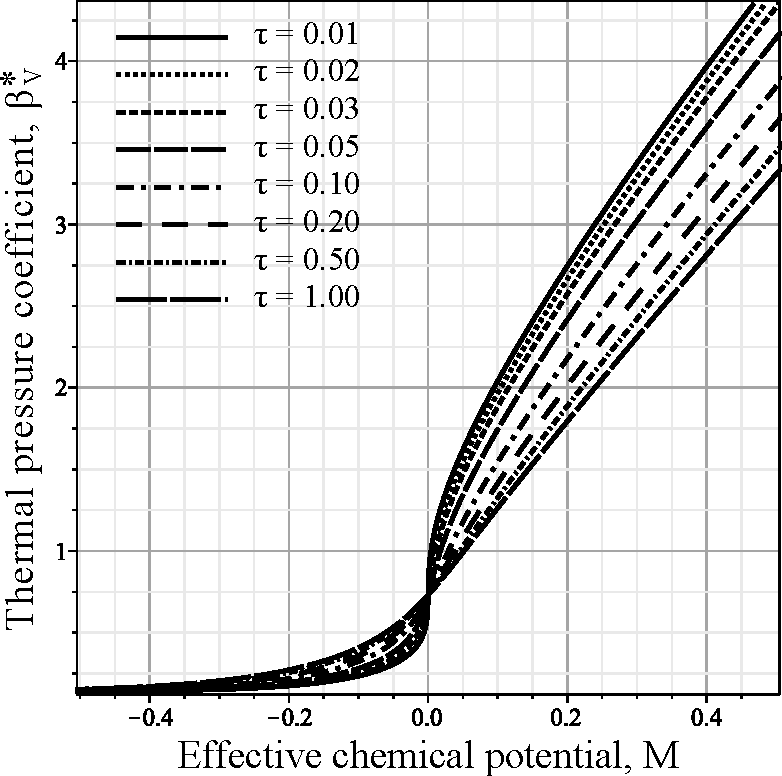
\includegraphics[width=0.5\textwidth]{f3b.pdf}
		\vskip-3mm\caption{The thermal pressure coefficient $\beta_V$ as a function of the effective chemical potential $M$ at different values of relative temperature $\tau > 0$ ($T > T_c$). 
		}\label{fig3b}
	\end{figure}
	\begin{figure}[h!]
		\centering 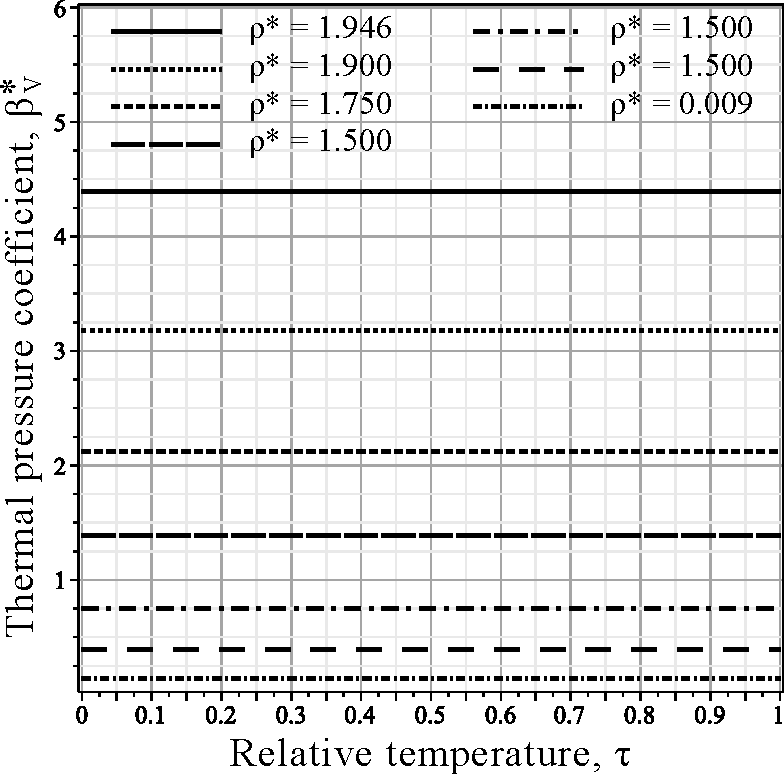
\includegraphics[width=0.5\textwidth]{f3c.pdf}
		\vskip-3mm\caption{The thermal pressure coefficient $\beta_V$ as a function of the relative temperature $\tau$ at different values of the density $\eta$. 
		}\label{fig3c}
	\end{figure}
	
	\subsection{Thermal expansion coefficient}
	The thermal expansion coefficient is defined by
	\begin{equation}
		\alpha_P = \frac{1}{V}\left(\frac{\partial V}{\partial T}\right)_{P,<N>}
	\end{equation}
	
	\begin{figure}[h!]
		\centering 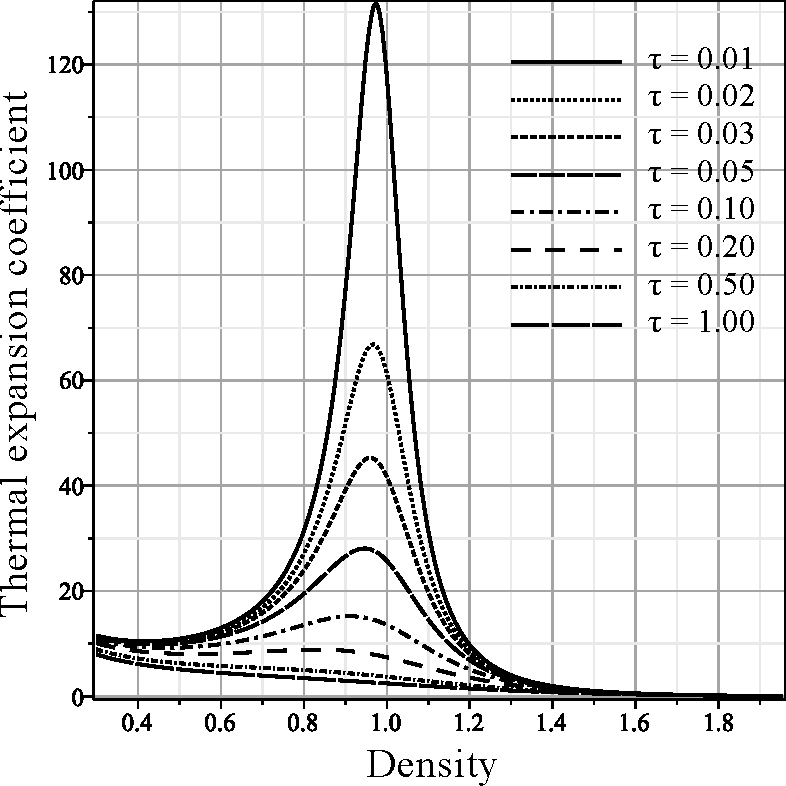
\includegraphics[width=0.5\textwidth]{f4a.pdf}
		\vskip-3mm\caption{The thermal expansion coefficient $\alpha_P$ as a function of the density $\bar n$ at different values of relative temperature $\tau > 0$ ($T > T_c$). 
		}\label{fig4a}
	\end{figure}
	
		\begin{figure}[h!]
		\centering 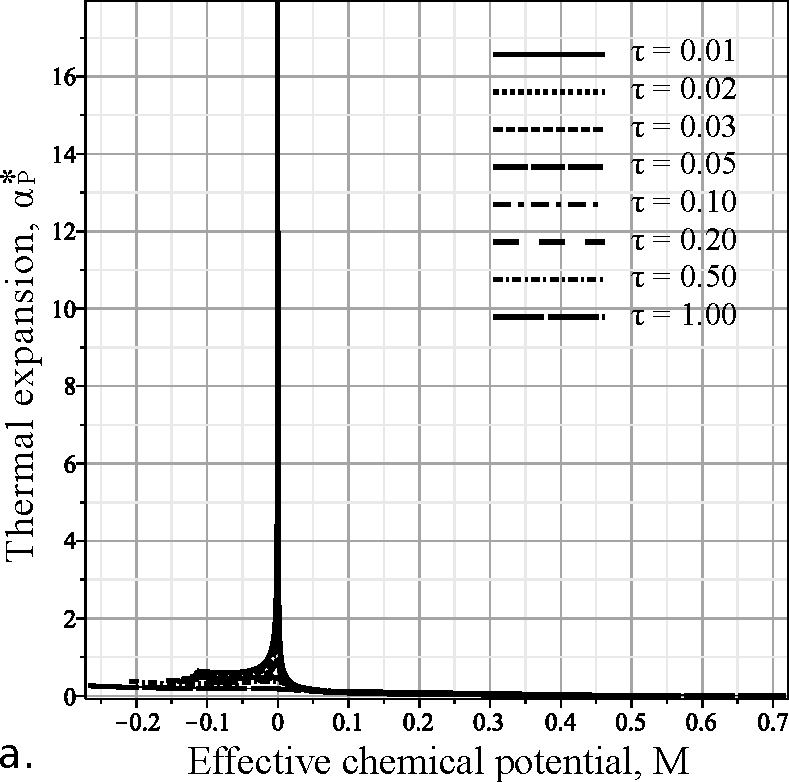
\includegraphics[width=0.45\textwidth]{f4b.pdf}
		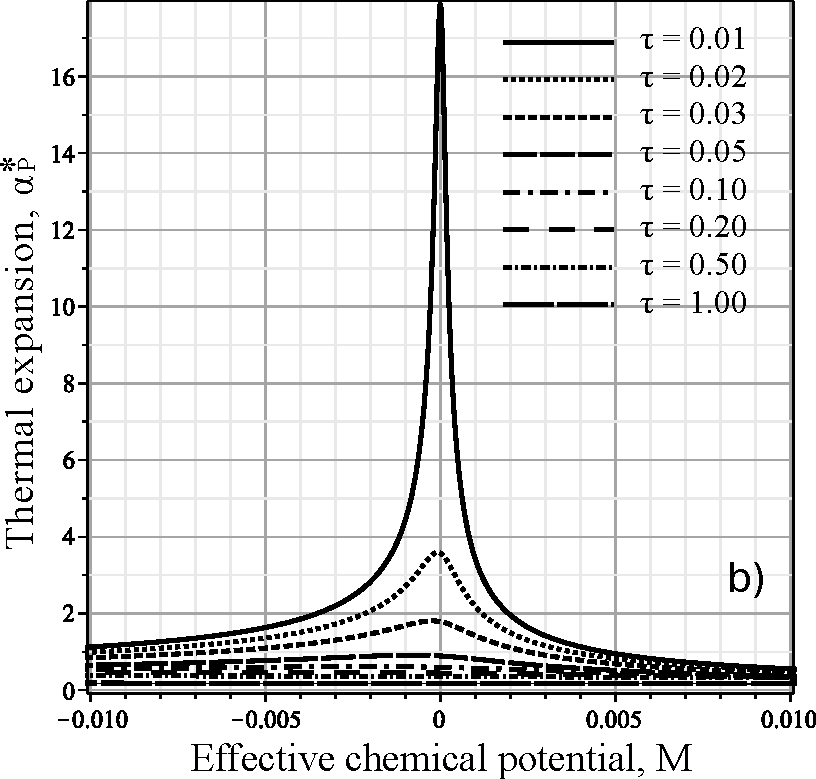
\includegraphics[width=0.475\textwidth]{f4c.pdf}
		\vskip-3mm\caption{The thermal expansion coefficient $\alpha_P$ as a function of the effective chemical potential $M$ for different temperatures $\tau = (T - T_c)/T_c$ at $T > T_c$. The two figures differ in the scale of $M$. The left-hand-side figure covers a wider range of $M$, while the right-hand-side one focuses on a range of $M$ around its critical value $0$.
		}\label{fig4b}
	\end{figure}
	
	\newpage 
	
	\section{Conclusions}
	Thermodynamic response functions, namely the isothermal compressibility, the thermal pressure coefficient, and the thermal expansion coefficient, are calculated for a many-particle system interacting through a modified Morse potential.
	
	%\bibliographystyle{cmpj} % still looking for the best style
	\bibliographystyle{elsarticle-num}
	%\bibliographystyle{unsrturl}
	%\bibliography{fluids_general,fluids_cv} % BibTeX / BibLaTeX should be used
	\bibliography{extracted}
	
\end{document}